\documentclass{minesbeamer}
\usepackage{graphicx}
\usepackage{hyperref}
%%%%%%%%%%%%%%%%%%%%%%%%%%%%%%%%%%%%%%%%%%%%%%%%%%%%%%%%%%%%%%%%%%%%%%%%%%%%%%
% \embedvideo{<poster or text>}{<video file (MP4+H264)>}
% \embedvideo*{...}{...}                     % auto-play
%%%%%%%%%%%%%%%%%%%%%%%%%%%%%%%%%%%%%%%%%%%%%%%%%%%%%%%%%%%%%%%%%%%%%%%%%%%%%%

\usepackage[bigfiles]{pdfbase}
\ExplSyntaxOn
\NewDocumentCommand\embedvideo{smm}{
  \group_begin:
  \leavevmode
  \tl_if_exist:cTF{file_\file_mdfive_hash:n{#3}}{
    \tl_set_eq:Nc\video{file_\file_mdfive_hash:n{#3}}
  }{
    \IfFileExists{#3}{}{\GenericError{}{File~`#3'~not~found}{}{}}
    \pbs_pdfobj:nnn{}{fstream}{{}{#3}}
    \pbs_pdfobj:nnn{}{dict}{
      /Type/Filespec/F~(#3)/UF~(#3)
      /EF~<</F~\pbs_pdflastobj:>>
    }
    \tl_set:Nx\video{\pbs_pdflastobj:}
    \tl_gset_eq:cN{file_\file_mdfive_hash:n{#3}}\video
  }
  %
  \pbs_pdfobj:nnn{}{dict}{
    /Type/RichMediaInstance/Subtype/Video
    /Asset~\video
    /Params~<</FlashVars (
      source=#3&
      skin=SkinOverAllNoFullNoCaption.swf&
      skinAutoHide=true&
      skinBackgroundColor=0x5F5F5F&
      skinBackgroundAlpha=0
    )>>
  }
  %
  \pbs_pdfobj:nnn{}{dict}{
    /Type/RichMediaConfiguration/Subtype/Video
    /Instances~[\pbs_pdflastobj:]
  }
  %
  \pbs_pdfobj:nnn{}{dict}{
    /Type/RichMediaContent
    /Assets~<<
      /Names~[(#3)~\video]
    >>
    /Configurations~[\pbs_pdflastobj:]
  }
  \tl_set:Nx\rmcontent{\pbs_pdflastobj:}
  %
  \pbs_pdfobj:nnn{}{dict}{
    /Activation~<<
      /Condition/\IfBooleanTF{#1}{PV}{XA}
      /Presentation~<</Style/Embedded>>
    >>
    /Deactivation~<</Condition/PI>>
  }
  %
  \hbox_set:Nn\l_tmpa_box{#2}
  \tl_set:Nx\l_box_wd_tl{\dim_use:N\box_wd:N\l_tmpa_box}
  \tl_set:Nx\l_box_ht_tl{\dim_use:N\box_ht:N\l_tmpa_box}
  \tl_set:Nx\l_box_dp_tl{\dim_use:N\box_dp:N\l_tmpa_box}
  \pbs_pdfxform:nnnnn{1}{1}{}{}{\l_tmpa_box}
  %
  \pbs_pdfannot:nnnn{\l_box_wd_tl}{\l_box_ht_tl}{\l_box_dp_tl}{
    /Subtype/RichMedia
    /BS~<</W~0/S/S>>
    /Contents~(embedded~video~file:#3)
    /NM~(rma:#3)
    /AP~<</N~\pbs_pdflastxform:>>
    /RichMediaSettings~\pbs_pdflastobj:
    /RichMediaContent~\rmcontent
  }
  \phantom{#2}
  \group_end:
}
\ExplSyntaxOff
%%%%%%%%%%%%%%%%%%%%%%%%%%%%%%%%%%%%%%%%%%%%%%%%%%%%%%%%%%%%%%%%%%%%%%%%%%%%%%
\graphicspath{{../graphics}}
\title{Theory and Methods for the Ferromagnetic Ising Model}
\subtitle{TTIC 31180}
\author[Jay Shen \and Mark Lee]{Jay Shen \and Mark Lee}
\date{5/21/2024} % or whatever the date you are presenting in is
% \copyrightnotice{Published by the American Institute of Aeronautics and Astronautics, Inc., with permission}

\begin{document}

\maketitle

\cutoc

\section{Review of the Ising Model}

\begin{frame}{What is an Ising Model?}
    \begin{columns}
        \begin{column}{0.6\textwidth}
            \begin{figure}
                \centering
                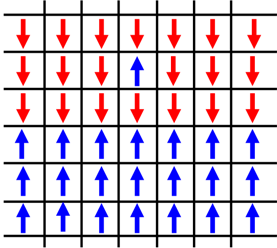
\includegraphics[height=0.7\textheight]{monte-carlo-ising-2.png}
            \end{figure}
        \end{column}
        \begin{column}{0.5\textwidth}
            \begin{itemize}
                \item The Ising model is used in statistical mechanics to describe ferromagnetism in materials.
                \item Each site on the lattice is associated with a spin, which represents the magnetic moment of an atom or molecule.
                \item The spins are subject to thermal fluctuations, causing them to flip between \{-1,1\}.
            \end{itemize}
        \end{column}
    \end{columns}
\end{frame}

\begin{frame}{Theory of the Ising Model}
    \begin{columns}
        \begin{column}{0.6\textwidth}
            \begin{itemize}
                \item A particle with magnetic moment $\vec{\mu}$ in an external magnetic field $\vec{B}$ has potential energy: $$U = -\vec{\mu}\cdot \vec{B}$$
                \item The magnetic moment also creates a magnetic field. The interaction between particles, denoted by exchange constants $J_{ij}$, also have potential energy: $$U = -J_{ij}\vec{\mu_1}\cdot\vec{\mu_2}$$
            \end{itemize}
        \end{column}
        \begin{column}{0.4\textwidth}
            \begin{figure}
                \centering
                \includegraphics[height=0.6\textheight]{3Dising.png}
            \end{figure}
        \end{column}
    \end{columns}
\end{frame}

\begin{frame}{Theory of the Ising Model cont.}
    \centering
    \begin{itemize}
        \item So now we have a collection of particles in the presence of an external magnetic field. The Hamiltonian, which specifies the total energy of the system, is defined by the sum of all pairwise and all magnetic field energies:$$E = -\frac{1}{2}\sum_{i,j}J_{ij}\vec{\mu_i}\cdot\vec{\mu_j}-\sum_i \vec{\mu_i}\cdot\vec{B}$$
        \item This is intractable, and we can simplify it through several assumptions. By coalescing constants,$$E=-J\sum_i\sum_{j\in adj(i)}\sigma_i\sigma_j -\sum_i \sigma_i B_i$$
    \end{itemize}
\end{frame}

\begin{frame}{Theory of the Ising Model cont.}
    \centering
    \begin{itemize}
        \item Following the Boltzmann distribution, the probability of some state $\vec{\sigma}$ at inverse temperature $\beta$ is:$$P(\vec{\sigma}) = \frac{1}{Z}e^{-\beta E(\vec{\sigma})}$$
    \end{itemize}
\end{frame}

\section{Inference Using the Ising Model}

\begin{frame}{Inference Using the Ising Model}
    \centering
    \begin{itemize}
        \item The motivation to perform inference on the ising model is to find the equilibrium distribution of spins that minimize the energy
        \item In our project, we tested two commonly used methods: MCMC and Belief Propagation.
    \end{itemize}
\end{frame}

\begin{frame}{Markov Chain Monte Carlo (MCMC)}
    \centering
    \begin{itemize}
        \item Sampling from the conditioned distribution corresponds to flipping some spins of some spin state $\vec{\sigma}$ to get a new spin state $\vec{\sigma}\textsc{\char13}$. If the new spin state is "more favorable" than the previous one, then we will flip to the new state. Thus, we can write the "probability" as: $$P_{\vec{\sigma} \to \vec{\sigma}\textsc{\char13}} = \frac{P(\vec{\sigma}\textsc{\char13})}{P(\vec{\sigma})}= e^{-\beta(E(\vec{\sigma}\textsc{\char13})-E(\vec{\sigma}))}$$ 
        \item In the case where only one spin $\sigma_i$ flips, we can write the energy difference in the exponential is $\displaystyle E(\vec{\sigma}\textsc{\char13})-E(\vec{\sigma}) = 2\sigma_i(J \sum_{j\in adj(i)} \sigma_j + B_i )$
    \end{itemize}
\end{frame}

\begin{frame}{Markov Chain Monte Carlo (MCMC) cont.}
    \centering
    \begin{itemize}
        \item The final expression is therefore: $$P_{\vec{\sigma} \to \vec{\sigma}\textsc{\char13}} = exp(-2\beta\sigma_i(J \sum_{j\in adj(i)} \sigma_j + B_i )))$$ 
        \item If the transition lowers the energy, accept it. Otherwise, accept it with probability $P_{\vec{\sigma} \to \vec{\sigma}\textsc{\char13}}$ 
    \end{itemize}
\end{frame}

\begin{frame}{Results of MCMC cont.}
    \centering
    \begin{figure}
    \href{https://drive.google.com/file/d/1rxzwuteOm7bDoig8iRXaAgJcydNfbF3O/view?usp=drive_link}{
\includegraphics[width = 5 cm, height = 5cm]{mcmc.png}}
    \end{figure}
\end{frame}

\begin{frame}{Belief Propagation}
    \centering
    The joint distribution of the Ising model is:
    \[
    P(\vec{\sigma}) = \exp \Bigr [ \beta \Bigr ( J\sum_i \sum_{j \in adj(i)} \sigma_i \sigma_j + \sum_i \sigma_i B_i \Bigr ) \Bigr ]
    \]
    This factors nicely as:
    \[
    P(\vec{\sigma}) = \prod_i \prod_{j \in adj(i)} \exp (J \beta \sigma_i \sigma_j) \cdot \prod_i \exp(\sigma_i \beta B_i)
    \]
    We can then define a factor graph of unary and pairwise potentials and use 
    belief propagation for inference. 
\end{frame}

\begin{frame}{Belief Propagation cont.}
    \centering
    \begin{figure}
    \href{https://drive.google.com/file/d/1EIDcN95oOABF0ZoCHTdMfJtEQk6D3qU0/view?usp=drive_link}{
\includegraphics[width = 5 cm, height = 5cm]{bp.png}}
    \end{figure}
\end{frame}

\begin{frame}{Sample-Based vs Belief Propagation}
    \begin{itemize}
        \item 
        Sample based inference has a hard time converging.
        \item 
        Belief propagation gives a distribution while MCMC gives a set of 
        samples.
        \item MCMC is more physically intuitive.
    \end{itemize}
\end{frame}

\begin{frame}{Discussion}
    \begin{itemize}        
        \item We simulate some phase transitions using MCMC:
        \centering

        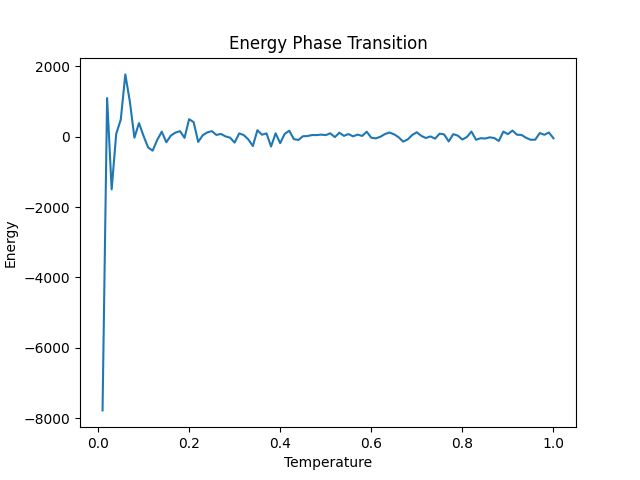
\includegraphics[height=0.6\textheight]{mcmc_phase.png}
    \end{itemize}
\end{frame}
% Q&A
\begin{frame}[standout]
    \Huge\textsc{Thank You}
    
    \vfill
    
    \LARGE\textsc{Questions?}
\end{frame}



\end{document}